\section{Sensores externos} \label{sec:sensores ecternos}
Los sensores externos se dividen en sensores de contacto y sensores sin contacto. 
\subsection{Sensores de contacto}
Son aquellos que necesitan tocar físicamente un objeto para detectar su presencia o medir una magnitud.
\subsection*{Interruptores de límite}
\begin{itemize}
	\item \textbf{¿Qué hacen?} Detectan la presencia o posición de un objeto cuando este activa un mecanismo mecánico.
	\item \textbf{Principio de funcionamiento:} Consisten en un brazo mecánico o palanca que, al ser presionado, acciona un interruptor eléctrico.
	\item \textbf{Aplicaciones:} Detección de posición en máquinas CNC y robots industriales.
	Protección en sistemas de seguridad (por ejemplo, cuando una puerta está abierta o cerrada).
	Sistemas de final de carrera en actuadores.
	\item \textbf{Ejemplo:} Interruptor de límite tipo microswitch, como los usados en impresoras 3D para el eje Z.
\end{itemize}
\begin{figure}[h]
	\centering
	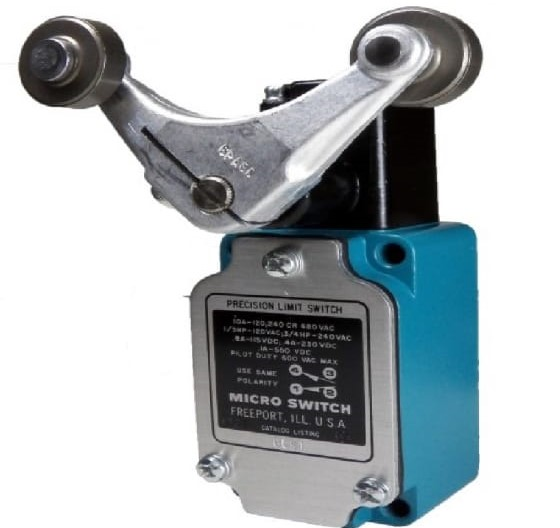
\includegraphics[width=0.3\linewidth]{img/sensor de limite}
	\label{fig:sensor de limite}
\end{figure}
\subsection*{Interruptores neumáticos}
\begin{itemize}
	\item \textbf{¿Qué hacen?} Detectan la presión de aire o vacío en un sistema neumático.
	\item \textbf{Principio de funcionamiento:} Usan un diafragma o válvula que se activa con cambios de presión.
	\item \textbf{Aplicaciones:} Control en sistemas de automatización neumática.
	Seguridad en prensas neumáticas y sistemas de frenado de emergencia.
	Sistemas de detección de flujo de aire.
	\item \textbf{Ejemplo:} Interruptor neumático utilizado en líneas de producción automatizadas.
\end{itemize}
\begin{figure}[h]
	\centering
	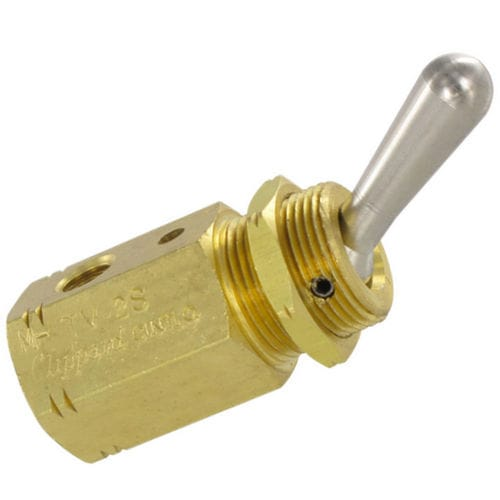
\includegraphics[width=0.3\linewidth]{img/sensor neumatico}
	\label{fig:sensor neumatico}
\end{figure}
\subsection*{Sensores piezoeléctricos}
\begin{itemize}
	\item \textbf{¿Qué hacen?} Detectan presión, fuerza o vibraciones y las convierten en señales eléctricas.
	\item \textbf{Principio de funcionamiento:} Se basan en el efecto piezoeléctrico, donde ciertos materiales generan un voltaje al ser sometidos a presión mecánica.
	\item \textbf{Aplicaciones:} Medición de impacto en pruebas de materiales.
	Sensores de vibración en maquinaria industrial.
	Micrófonos y captadores de sonido.
	\item \textbf{Ejemplo:} Sensores piezoeléctricos usados en guitarras eléctricas para captar sonido.
\end{itemize}
\begin{figure}[h]
	\centering
	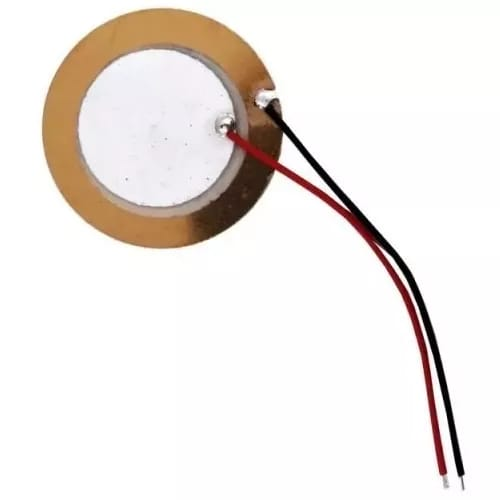
\includegraphics[width=0.3\linewidth]{img/sensor piezoelectrico}
	\label{fig:sensor piezoelectrico}
\end{figure}
\subsection*{Transductores de presión}
\begin{itemize}
	\item \textbf{¿Qué hacen?} Miden la presión de un fluido (líquido o gas) y la convierten en una señal eléctrica.
	\item \textbf{Principio de funcionamiento:} Usan galgas extensométricas o elementos piezoeléctricos para medir la deformación causada por la presión.
	\item \textbf{Aplicaciones:} Monitoreo de presión en sistemas hidráulicos y neumáticos.
	Control de presión en motores y sistemas de refrigeración.
	Aplicaciones médicas (como en esfigmomanómetros digitales).
	\item \textbf{Ejemplo:} Sensor de presión MPX5700 usado en sistemas de control de presión.
\end{itemize}
\begin{figure}[h]
	\centering
	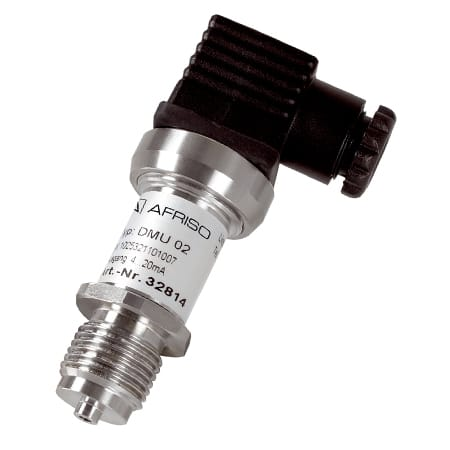
\includegraphics[width=0.3\linewidth]{img/transductor de presion}
	\label{fig:transductor de presion}
\end{figure}
\subsection{Sensores sin contacto}
Detectan la presencia, distancia o características de un objeto sin tocarlo.
\subsection*{Sensores de proximidad}
\begin{itemize}
	\item \textbf{¿Qué hacen?} Detectan la presencia de un objeto cercano sin contacto físico.
	\item \textbf{Tipos y funcionamiento:}
	
	\texttt{Inductivos:} Detectan objetos metálicos mediante un campo electromagnético.
	
	\texttt{Capacitivos:} Detectan objetos metálicos y no metálicos mediante cambios en la capacitancia.
	
	\texttt{Ópticos:} Usan luz infrarroja o láser para detectar objetos.
	\item \textbf{Aplicaciones:} Detección de piezas en bandas transportadoras.
	Sistemas de seguridad en maquinaria.
	Sensores de aparcamiento en automóviles.
	\item \textbf{Ejemplo:} Sensor inductivo LJ12A3-4-Z/BX usado en impresoras 3D.
\end{itemize}
\begin{figure}[h]
	\centering
	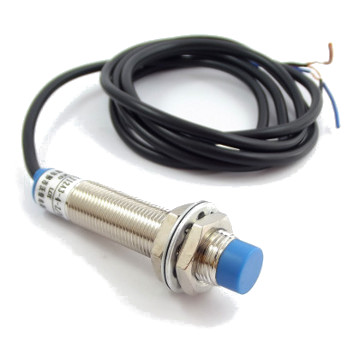
\includegraphics[width=0.3\linewidth]{img/sensor de proximidad}
	\label{fig:sensor de proximidad}
\end{figure}
\subsection*{Sensores de efecto Hall}
\begin{itemize}
	\item \textbf{¿Qué hacen?} Detectan la presencia de campos magnéticos.
	\item \textbf{Principio de funcionamiento:} Se basan en el efecto Hall, que genera una diferencia de voltaje en un material conductor cuando es atravesado por un campo magnético.
	\item \textbf{Aplicaciones:} Sensores de velocidad en motores.
	Controles de proximidad en robótica.
	Medición de corriente en circuitos eléctricos.
	\item \textbf{Ejemplo:} Sensor de efecto Hall A3144 para detectar imanes.
\end{itemize}
\begin{figure}[h]
	\centering
	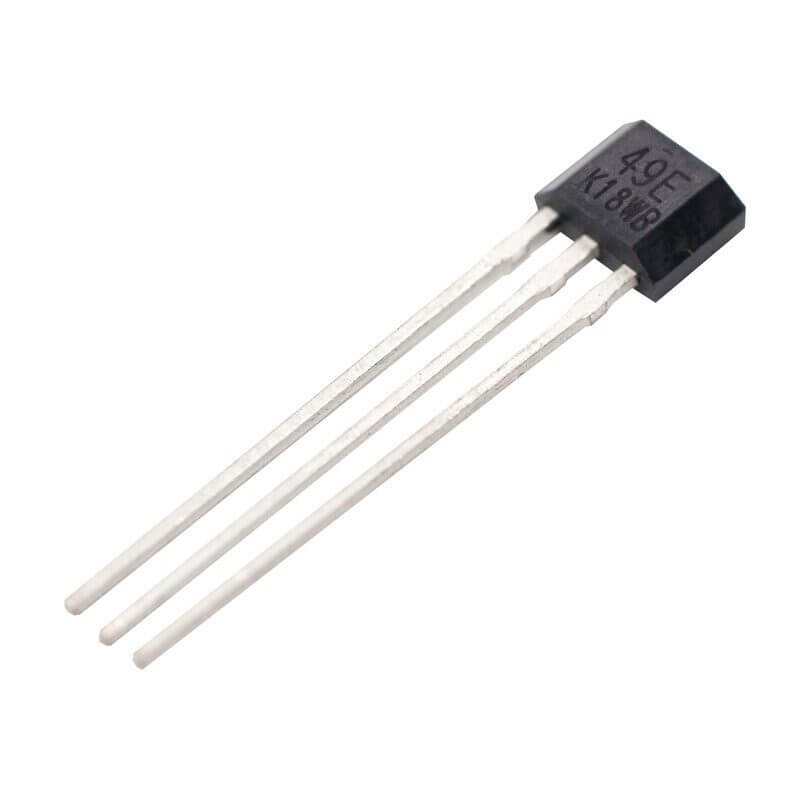
\includegraphics[width=0.3\linewidth]{img/sensor de efecto hall}
	\label{fig:sensor de efecto hall}
\end{figure}
\subsection*{Sensores de microondas}
\begin{itemize}
	\item \textbf{¿Qué hacen?} Detectan movimiento mediante la emisión y recepción de ondas electromagnéticas de alta frecuencia.
	\item \textbf{Principio de funcionamiento:} Utilizan el efecto Doppler: cuando un objeto se mueve, la frecuencia reflejada cambia, lo que permite detectar su presencia y velocidad.
	\item \textbf{Aplicaciones:} Sensores de movimiento en alarmas de seguridad.
	Detección de vehículos en semáforos inteligentes.
	Sensores de radar en autos autónomos.
	\item \textbf{Ejemplo:} Sensor de microondas RCWL-0516 usado en sistemas de iluminación automática.
\end{itemize}
\begin{figure}[h]
	\centering
	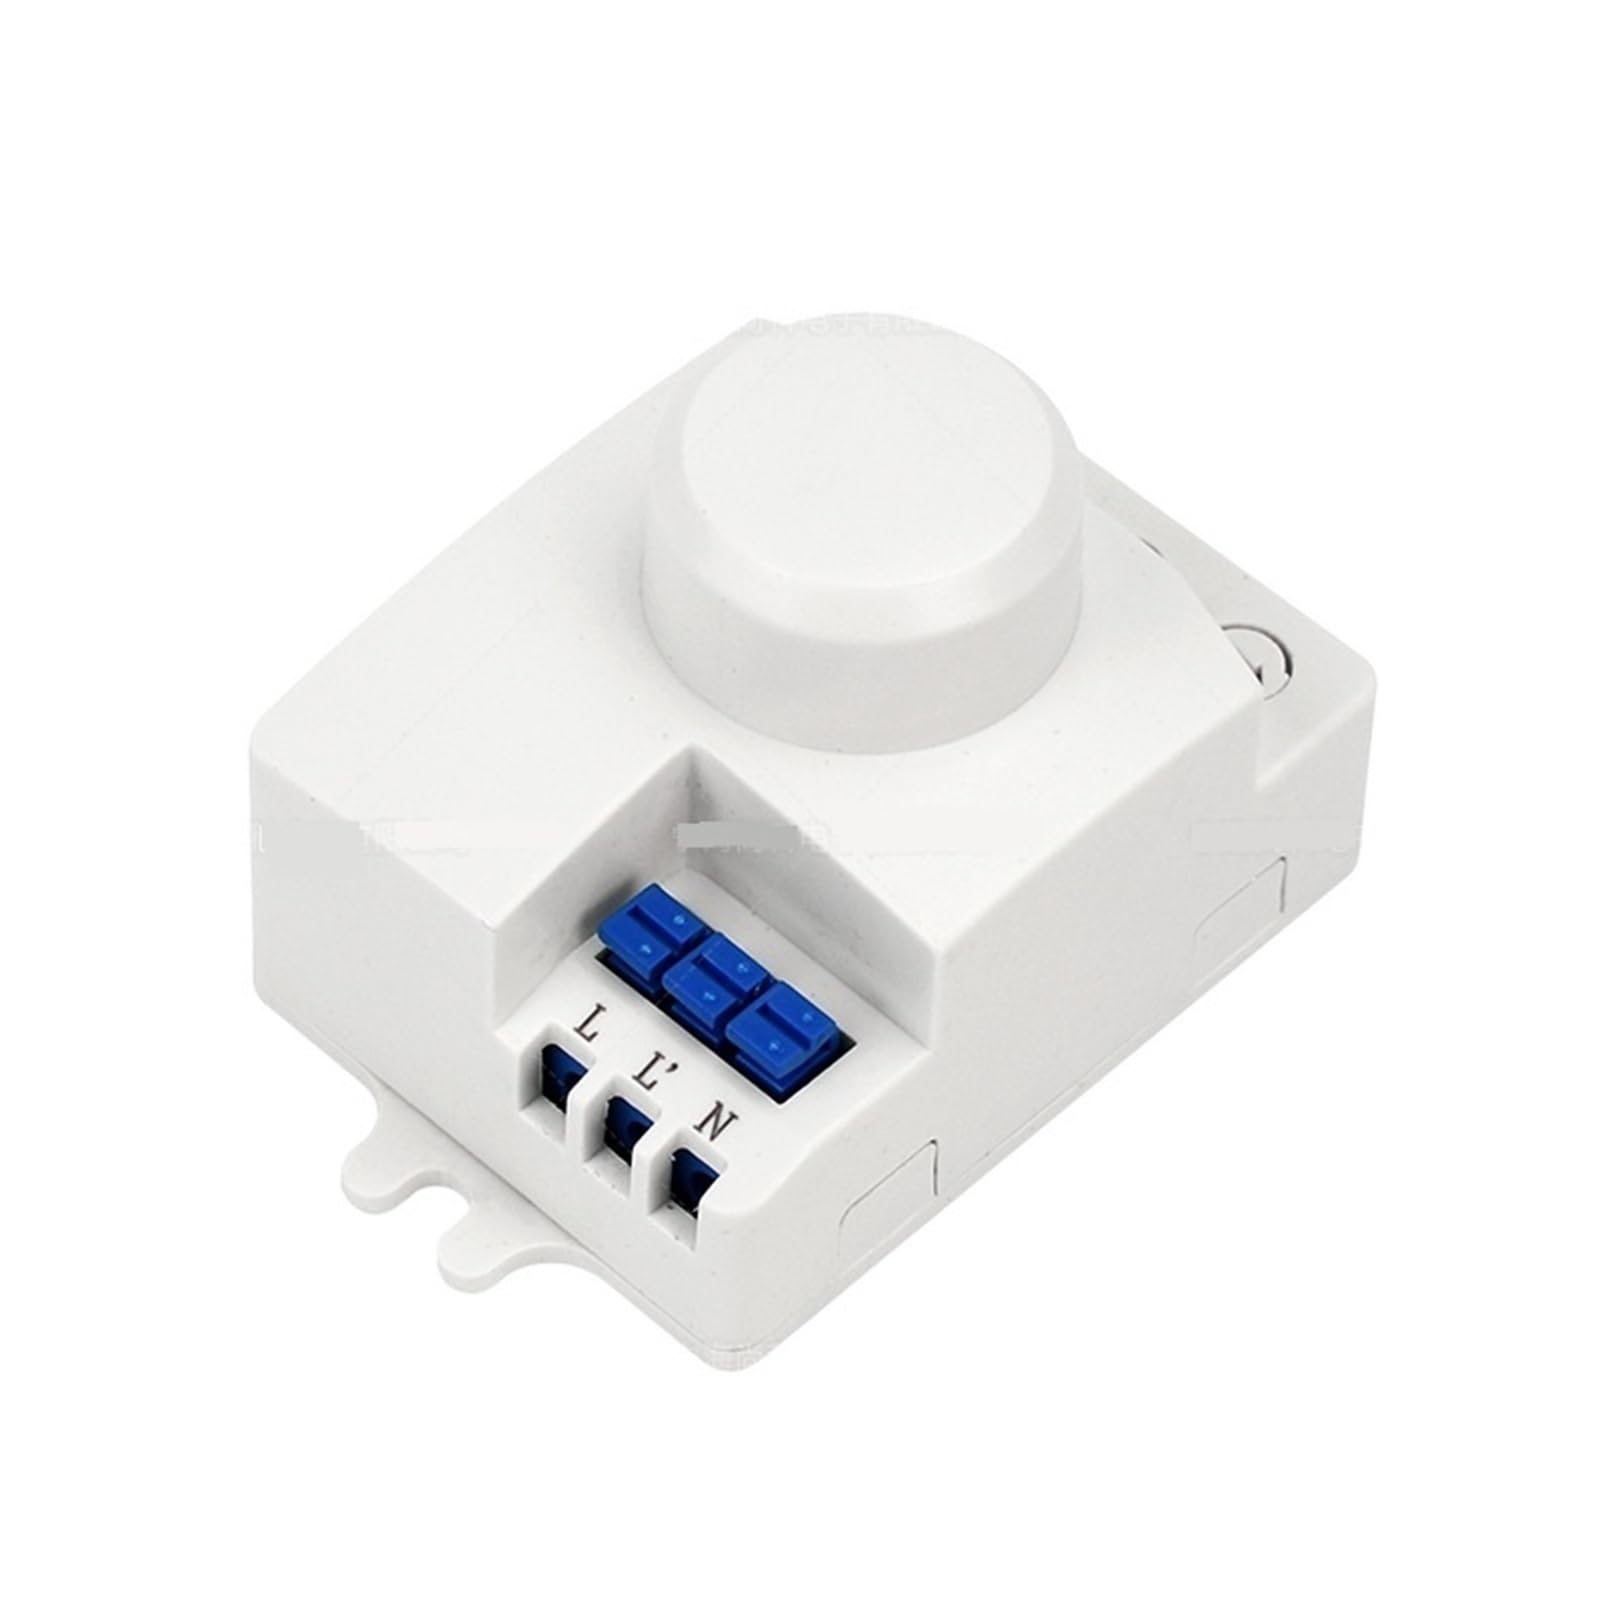
\includegraphics[width=0.3\linewidth]{img/sensor de microondas}
	\label{fig:sensor de microondas}
\end{figure}
\subsection*{Sensores ultasónicos}
\begin{itemize}
	\item \textbf{¿Qué hacen?} Capturan imágenes y procesan información visual.
	\item \textbf{Principio de funcionamiento:} Utilizan cámaras con algoritmos de procesamiento de imagen para detectar formas, colores y movimientos.
	\item \textbf{Aplicaciones:} Inspección de calidad en líneas de producción.
	Reconocimiento facial en seguridad.
	Navegación de robots autónomos.
	\item \textbf{Ejemplo:} Cámara Intel RealSense para visión 3D.
\end{itemize}
\begin{figure}[h]
	\centering
	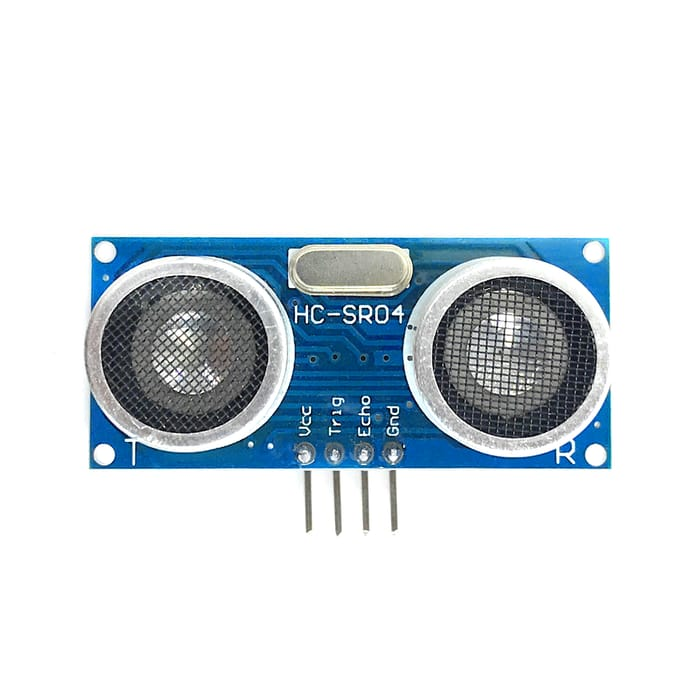
\includegraphics[width=0.3\linewidth]{img/sensor ultrasonico}
	\label{fig:sensor ultrasonico}
\end{figure}
\subsection*{Sensores láser}
\begin{itemize}
	\item \textbf{¿Qué hacen?} Miden distancias con alta precisión mediante un haz de luz láser.
	\item \textbf{Principio de funcionamiento:} Utilizan el tiempo de vuelo (ToF) de un pulso láser para calcular la distancia.
	\item \textbf{Aplicaciones:} Mapeo 3D en drones y vehículos autónomos.
	Medición de distancias en topografía.
	Sensores de seguridad en máquinas industriales.
	\item \textbf{Ejemplo:} Sensor LiDAR TFmini usado en robots para navegación autónoma.
\end{itemize}
\begin{figure}[h]
	\centering
	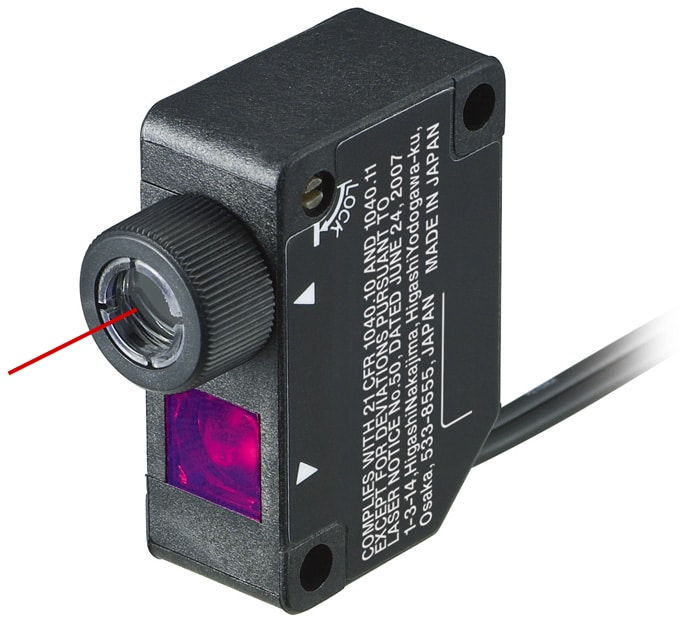
\includegraphics[width=0.3\linewidth]{img/sensor laser}
	\label{fig:sensor laser}
\end{figure}
\subsection*{Sensores de visión}
\begin{itemize}
	\item \textbf{¿Qué hacen?} Detectan movimiento mediante la emisión y recepción de ondas electromagnéticas de alta frecuencia.
	\item \textbf{Principio de funcionamiento:} Utilizan el efecto Doppler: cuando un objeto se mueve, la frecuencia reflejada cambia, lo que permite detectar su presencia y velocidad.
	\item \textbf{Aplicaciones:} Sensores de movimiento en alarmas de seguridad.
	Detección de vehículos en semáforos inteligentes.
	Sensores de radar en autos autónomos.
	\item \textbf{Ejemplo:} Sensor de microondas RCWL-0516 usado en sistemas de iluminación automática.
\end{itemize}

\newcounter{actividad} % Define un contador llamado "actividad"
\begin{longtable}{|c|p{10cm}|c|} % Define anchos específicos
	\caption{Resumen de los tipos de sensores externos.} \label{tab:ejemplo_tabla} \\
	\hline
	\textbf{Sensor} & \textbf{¿Como funciona?} & \textbf{Aplicaciones} \\
	\hline
	\endfirsthead
	\multicolumn{3}{c}{{\tablename\ \thetable{} -- continuación}} \\
	\hline
	\textbf{Sensor} & \textbf{¿Cómo funciona} & \textbf{Aplicaciones} \\
	\hline
	\endhead
	\hline \multicolumn{3}{r}{{Continúa en la siguiente página...}} \\
	\hline
	\endfoot
	\hline
	\endlastfoot
	% Contenido de la tabla
	Interruptores de límite. & Se activa al contacto. & Máquinas CNC, sistemas de seguridad. \\
	Interruptores neumáticos. & Detectan presión del aire. & Sistemas neumáticos y de frenos. \\
	Sensores piezoeléctricos. & Generan voltaje al recibir presión. & Detección de vibraciones e impacto. \\
	Transductores de presión. & Convierten presión en señal eléctrica. & Control en motores y sistemas hidráulicos. \\
	Sensores de proximidad. & Detectan objetos cercanos sin contacto. & Detección de piezas, sistemas de aparcamiento. \\
	Sensores de efecto Hall. & Detectan campos magnéticos. & Sensores de velocidad, control de motores. \\
	Sensores de microondas & Usa ondas electromagnéticas. & Alarmas, deteccion de vehiculos. \\
	Sensores ultrasónicos. & Usan ondas de sonido para medir distancias. & Robótica, aparcamiento de autos. \\
	Sensores láser. & Emplean luz laser para medir distancias. & LiDAR, seguridad industrial. \\
	Sensores de visión. & Capturan y procesan imágenes. & Reconocimiento facial, inspección de calidad. \\
\end{longtable}